\chapter{Results}
\label{ch:results}

\section{Evaluation setup}

For our evaluation, we simulate a MemPool \gls{soc} in its \emph{MinPool} (16-core) configuration
using the Verilator~\cite{verilator} simulator. Additionally, we increase the stack size for each
core to 1024 bytes to accommodate the higher stack usage of the new runtime, and disable the
\texttt{Xpulp} instructions, since they are not fully supported when compiling with LLVM.

In order to compare the performance of the new runtime against the previous one, we run a part of
the existing benchmarks available in the MemPool
repository\footnote{\url{https://github.com/pulp-platform/mempool}} using both of them.

For correctness, we run the set of tests also provided in the MemPool repository, however, we adapt
them to use the new testing framework described in the following section. Additionally, we add new
tests for the \texttt{teams} and \texttt{sections} constructs, which we describe in more detail in
\cref{sec:correctness}.

\subsection{Testing Framework}
\label{subsec:testing-framework}

The testing framework consists of a small set of C preprocessor macros that allow us to make
assertions, define test cases and run them. It is inspired by \citeauthor{minunit}'s minimal testing
framework~\cite{minunit}.

It is comprised of the following macros:

\begin{itemize}
	\item \texttt{ASSERT_TRUE(condition, error_message)}: Checks that \texttt{condition} evaluates to
	      \texttt{true}. If it does not, it prints \texttt{error_message} and fails the test.
	\item \texttt{ASSERT_EQ(left, right)}: Checks that \texttt{left} is equal to \texttt{right}. If
	      it is not, it prints an error message and fails the test.
	\item \texttt{ASSERT_NEQ(left, right)}: Checks that \texttt{left} is not equal to \texttt{right}.
	      If it is, it prints an error message and fails the test.
	\item \texttt{EXPECT_TRUE(condition, error_message)}: Similar to \texttt{ASSERT_TRUE}, but does
	      not fail the test if the condition is not met, it only prints the error message.
	\item \texttt{TEST(testname)}: Defines a new test with the name \texttt{testname} and adds it to
	      the list of tests to be run.
	\item \texttt{RUN_TEST(testname)}: Runs the test \texttt{testname}.
	\item \texttt{RUN_ALL_TESTS()}: Runs all tests defined in the test suite.
	\item \texttt{PRINT_TEST_RESULTS()}: Prints the results of the test suite (i.e., how many tests
	      were run and how many failed).
\end{itemize}

When printing, the framework includes easy to parse markers to the output such as, \texttt{[FAIL]}
or \texttt{[SUCCESS]}, which can be used by, e.g., a python script to run multiple tests in
succession and automatically show the results to the user.

\section{Correctness}
\label{sec:correctness}

Our implementation passes all of the correctness tests provided in the MemPool repository, as well as
the new tests described in the following sections.

\subsection{\texttt{teams} Construct}

The test shown in \cref{lst:test-teams-distribute} checks that the \texttt{teams distribute}
construct correctly distributes the iterations of the loop across the teams. It does so by checking
that the team number is correct for each iteration. It also checks that the number of teams matches
the number of requested teams by comparing the value returned by \texttt{omp\_get\_num\_teams()} to
the expected value (4).

\begin{lstlisting}[language=C, caption={test_teams_distribute}, label={lst:test-teams-distribute}]
TEST(test_teams_distribute) {
  for (int rep = 0; rep < REPETITIONS; rep++) {
    int num_teams = 0;
    int team_num[12];

#pragma omp teams distribute num_teams(4)
    for (int i = 0; i < 12; i++) {
      team_num[i] = omp_get_team_num();

      if (omp_get_team_num() == 0) {
        num_teams = omp_get_num_teams();
      }
    }

    for (int i = 0; i < 12; i++) {
      ASSERT_EQ(team_num[i], i / 3);
    }

    ASSERT_EQ(num_teams, 4);
  }
}
\end{lstlisting}

The test shown in \cref{lst:test-teams-reduce} checks that each team is able to work independently
by performing a reduction onto a team-local variable. The result of each reduction is then compared
against the expected value (32).

\begin{lstlisting}[language=C, caption={tests_teams_reduce}, label={lst:test-teams-reduce}]
TEST(test_teams_reduce) {
  for (int rep = 0; rep < REPETITIONS; rep++) {
    int sum[4];

#pragma omp teams num_teams(4)
    {
      int local_sum = 0;

#pragma omp parallel for reduction(+ : local_sum)
      for (int i = 0; i < 32; i++) {
        local_sum += 1;
      }

      sum[omp_get_team_num()] = local_sum;
    }

    for (int i = 0; i < 4; i++) {
      ASSERT_EQ(sum[i], 32);
    }
  }
}
\end{lstlisting}

Finally, the test shown in \cref{lst:test-teams-barrier} checks that barriers work correctly within
teams and don't affect other teams. It does so by performing an independent barrier test in each
team, that checks that the barrier is functional.

\begin{lstlisting}[language=C, caption={test_teams_barrier}, label={lst:test-teams-barrier}]
TEST(test_teams_barrier) {
  for (int rep = 0; rep < REPETITIONS; rep++) {
    int results[2];
#pragma omp teams num_teams(2)
    {
      uint32_t team_num = omp_get_team_num();
      int result = 0;

#pragma omp parallel
      {
        uint32_t rank = omp_get_thread_num();
        if (rank == 1) {
          mempool_wait(1000);
          result = 3;
        }
#pragma omp barrier

        if (rank == 2) {
          results[team_num] = result;
        }
      }
    }

    ASSERT_EQ(results[0], 3);
    ASSERT_EQ(results[1], 3);
  }
}
\end{lstlisting}

\subsection{\texttt{sections} Construct}

The test shown in \cref{lst:test-sections} checks that the \texttt{sections} construct correctly
distributes the sections across the threads. It does so by checking that each section is executed by
a different thread.

\begin{lstlisting}[language=C, caption={test_omp_parallel_sections}, label={lst:test-sections}]
TEST(test_omp_parallel_sections) {
  for (int rep = 0; rep < REPETITIONS; rep++) {
    uint32_t section_1 = 0;
    uint32_t section_2 = 0;

#pragma omp parallel sections
    {

#pragma omp section
      { section_1 = omp_get_thread_num(); }

#pragma omp section
      { section_2 = omp_get_thread_num(); }
    }

    ASSERT_NEQ(section_1, section_2);
  }
}
\end{lstlisting}

\section{Performance}

To account for performance differences that arise purely from using different compilers, we compare
the performance of the new runtime against the previous one in two different ways:

First, we obtain the speedup of running a given workload in parallel versus sequentially with the
same compiler, and compare this across runtimes. This way, the effect of a more performant
compilation output will be mitigated, since the speedup is calculated relative to the sequential
baseline. The results of this approach will be discussed in \cref{subsec:speedup}.

Then, we look at the cost of specific runtime operations (e.g., barriers, startup time, etc.)
and compare them across runtimes as well. This way we can isolate individual components and see
if any of them could benefit from further optimizations. The results of this approach will be
discussed in \cref{subsec:runtime-overhead}.

\subsection{Speedup}
\label{subsec:speedup}

\subsubsection{Sparse Matrix-Vector Multiplication}

In this benchmark, we perform \gls{spvm}, where the matrix is stored in
\gls{csr} format. It has 512 columns and we vary the number of rows from 1 to 512.

\begin{figure}[h]
	\centering
	\begin{minipage}{0.49\textwidth}
		\centering
		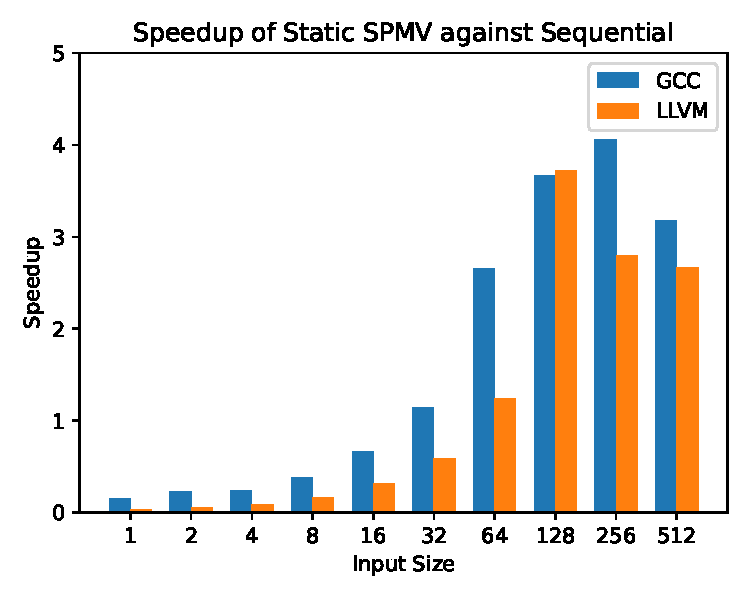
\includegraphics[width=\linewidth]{./fig/benchmarks/spvm_speedup_static.pdf}
		\caption{Static SPVM Speedup.}%
		\label{fig:spvm-static-speedup}
	\end{minipage}\hfill
	\begin{minipage}{0.49\textwidth}
		\centering
		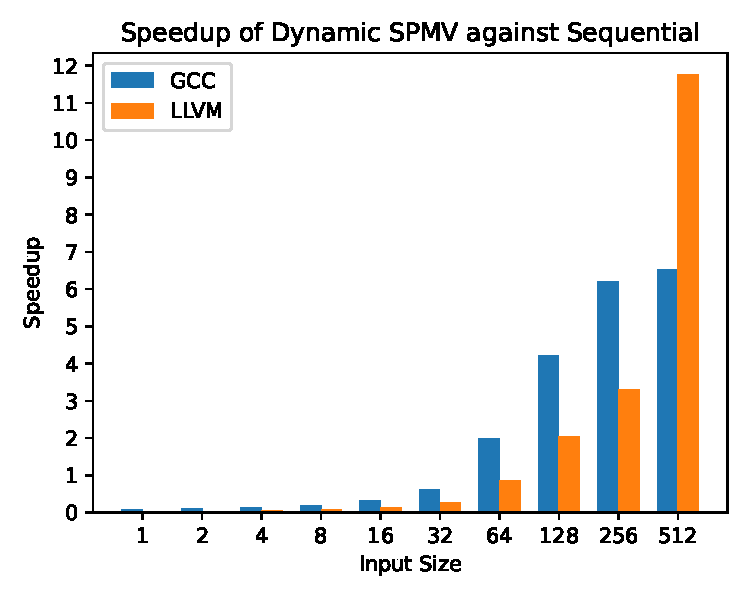
\includegraphics[width=\linewidth]{./fig/benchmarks/spvm_speedup_dynamic.pdf}
		\caption{Dynamic SPVM Speedup.}%
		\label{fig:spvm-dynamic-speedup}
	\end{minipage}
\end{figure}

\subsubsection{Matrix-Matrix Multiplication}

In this benchmark, we perform \gls{mmm} of square matrices, where we vary the
size of both matrices from 1 to 32.

\begin{figure}[h]
	\centering
	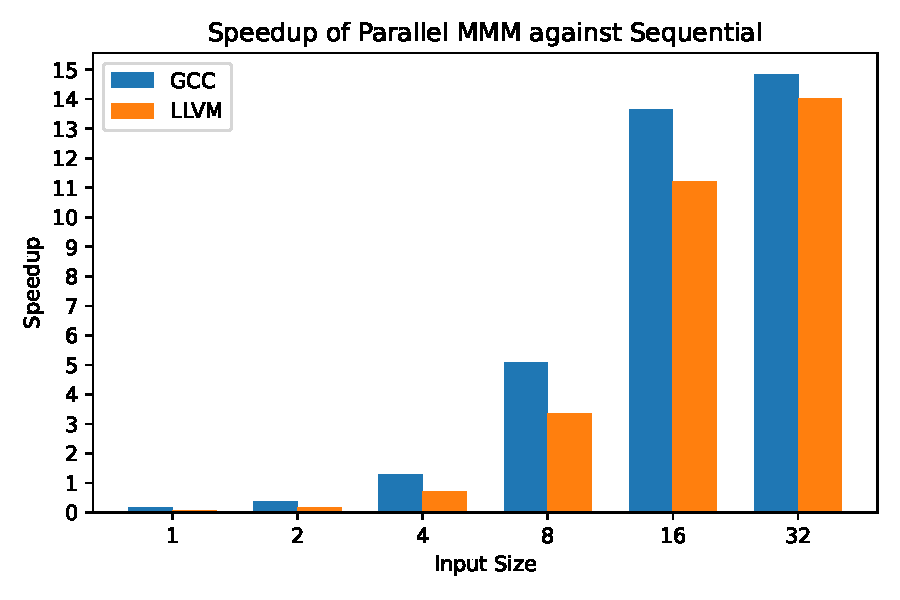
\includegraphics[width=.59\linewidth]{./fig/benchmarks/mm_speedup.pdf}
	\caption{Matrix-Matrix Multiplication Speedup.}%
	\label{fig:mm-speedup}
\end{figure}

\subsubsection{Dot Product}

In this benchmark, we perform the dot product of two vectors of size 1 to 2048.

\begin{figure}[h]
	\centering
	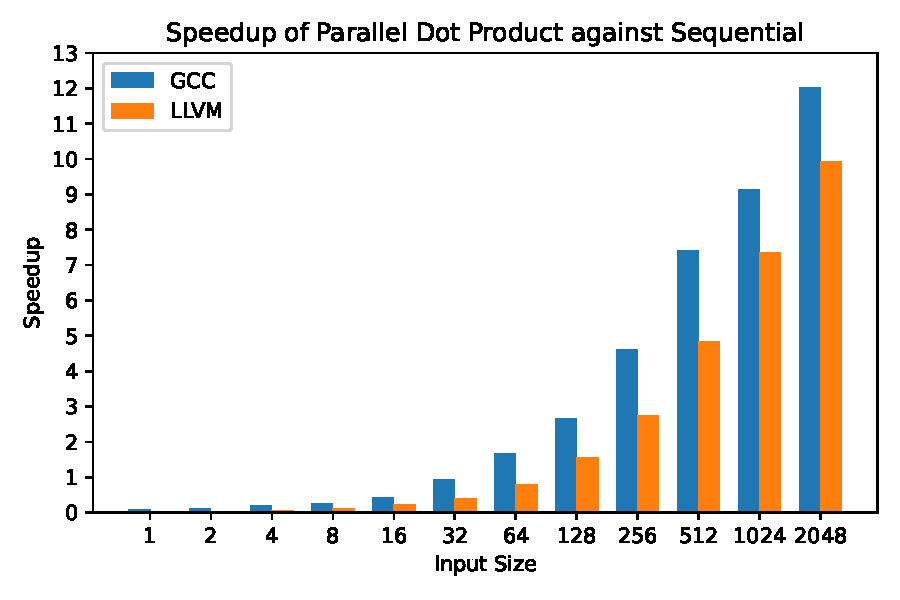
\includegraphics[width=.59\linewidth]{./fig/benchmarks/dotp_speedup.pdf}
	\caption{Dot Product Speedup.}%
	\label{fig:dotp-speedup}
\end{figure}

\subsection{Runtime Overhead}
\label{subsec:runtime-overhead}

\subsubsection{Startup Time}

We measure the runtime startup time using the benchmark shown in \cref{lst:benchmark-startup-time}. A
timer is started before executing the parallel region and stopped by the master thread inside a
master construct. We do this because the master thread is the one that performs the fork and we can
therefore know that when the master thread stops the timer, all of the other threads have at least
been initialized. The duration is averaged across 100 repetitions.

\begin{lstlisting}[language=C, caption={Startup Time Benchmark},
                   label={lst:benchmark-startup-time}]
void startup_time() {

  uint32_t duration = 0;

  for (int i = 0; i < REPETITIONS; i++) {

    mempool_timer_t cycles = mempool_get_timer();
    mempool_start_benchmark();

    #pragma omp parallel
    {

      #pragma omp master
      {
        mempool_stop_benchmark();
        cycles = mempool_get_timer() - cycles;
        duration += cycles;
      }
    }
  }

  printf("Startup time duration: %d\n", duration / REPETITIONS);
}
\end{lstlisting}

The results of the benchmarks are shown in \cref{tbl:benchmark-startup-time}, where we can see that
the new runtime has a startup time that is more than twice as long as the previous one.

\begin{table}[h]
	\centerfloat
	\begin{tabular}{ r r r r }
		\toprule
		\textbf{Runtime} & \textbf{Startup Time (cycles)} & \textbf{Speedup (vs. GCC)} \\
		\midrule
		GCC              & 154                            & 1                          \\
		LLVM             & 355                            & 0.43                       \\
		\bottomrule
	\end{tabular}
	\caption{Startup Time Benchmark Results.}%
	\label{tbl:benchmark-startup-time}
\end{table}

\subsubsection{Barrier}

In this benchmark, we measure the number of cycles it takes to execute an increasing number of
barriers, as shown in \cref{lst:benchmark-barrier}.

\begin{lstlisting}[language=C, caption={Barrier Benchmark},
                   label={lst:benchmark-barrier}]
int main() {
#pragma omp parallel
  {
    unsigned int counter = 0;
    unsigned int cycles = 0;
    unsigned int start_time = 0;

    for (int i = 1; i < MAX_BARRIERS + 1; i++) {

#pragma omp barrier

      start_time = mempool_get_timer();
      mempool_start_benchmark();

      for (int j = 0; j < i; j++) {
#pragma omp barrier
        counter++;
      }

      mempool_stop_benchmark();
      cycles = mempool_get_timer() - start_time;

#pragma omp single
      printf("%d barriers: %d cycles\n", i, cycles);
    }
  }

  return 0;
}
\end{lstlisting}

As expected, the number of cycles increases linearly with the number of barriers, as shown in
\cref{fig:barrier-benchmark-cycles}. The execution time of a barrier using the new runtime is about
18\% faster than with old one, as shown in \cref{fig:barrier-benchmark-speedup}. \todo{Explain why
	for one barrier it is faster}

\begin{figure}[h]
	\centering
	\begin{minipage}{0.49\textwidth}
		\centering
		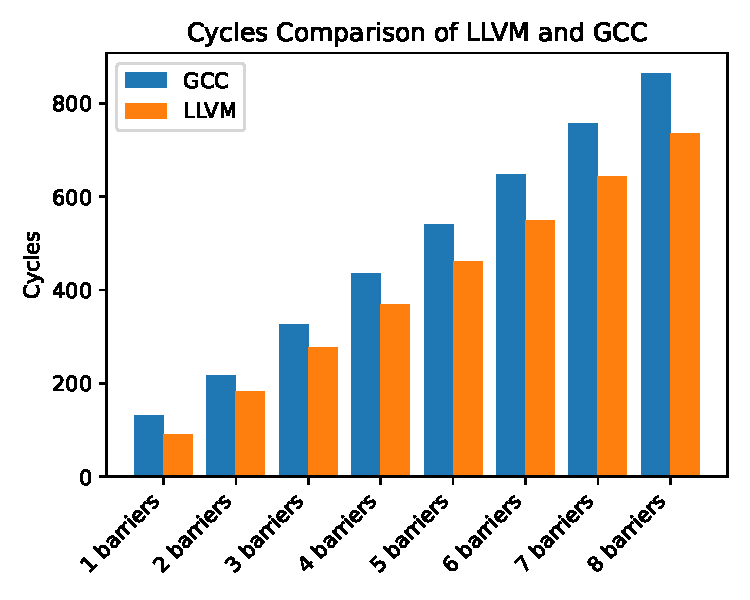
\includegraphics[width=\linewidth]{./fig/benchmarks/barrier_benchmark_cycles.pdf}
		\caption{Barrier Benchmark Cycles.}%
		\label{fig:barrier-benchmark-cycles}
	\end{minipage}\hfill
	\begin{minipage}{0.49\textwidth}
		\centering
		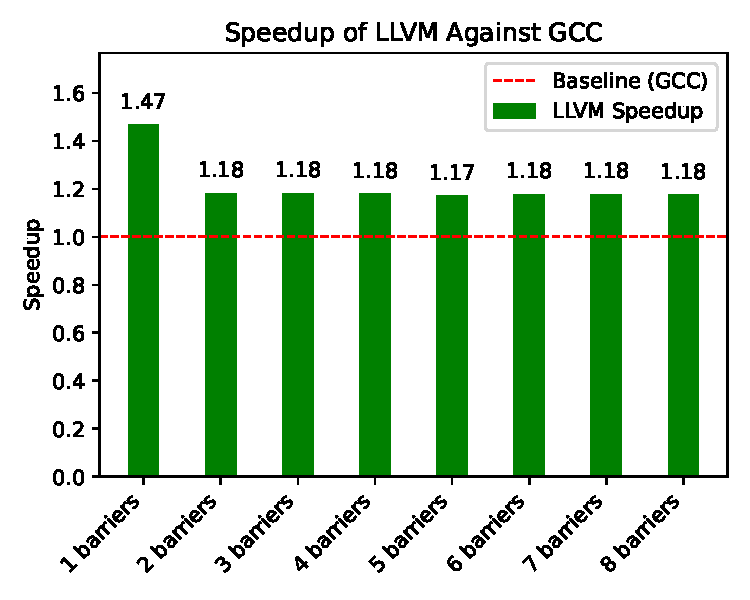
\includegraphics[width=\linewidth]{./fig/benchmarks/barrier_benchmark_speedup.pdf}
		\caption{Barrier Benchmark Speedup.}%
		\label{fig:barrier-benchmark-speedup}
	\end{minipage}
\end{figure}

\subsubsection{Critical Section}

In this benchmark, we measure the number of cycles it takes to execute a \texttt{critical} section,
as shown in \cref{lst:benchmark-critical}. The timer is started before the critical section and
stopped right after it is done executing. The master thread then aggregates the duration of each run
to finally print the average over 100 repetitions.

\begin{lstlisting}[language=C, caption={Critical Benchmark},
                   label={lst:benchmark-critical}]
void omp_parallel_critical() {
  uint32_t num_cores = mempool_get_core_count();
  uint32_t duration = 0;

  for (int i = 0; i < 100; i++) {

#pragma omp parallel num_threads(num_cores)
    {
      mempool_timer_t cycles = mempool_get_timer();
      mempool_start_benchmark();

#pragma omp critical
      { result += 100; }

      mempool_stop_benchmark();
      cycles = mempool_get_timer() - cycles;

#pragma omp master
      { duration += cycles; }
    }
  }

  printf("OMP Critical Duration: %d\n", duration / 100);
}
\end{lstlisting}

As shown in \cref{tbl:critical}, the new runtime achieves comparable performance in this benchmark,
needing less than 10 extra cycles to execute a critical section.

\begin{table}[h]
	\centerfloat
	\begin{tabular}{ r r r r }
		\toprule
		\textbf{Runtime} & \textbf{Critical Section (cycles)} & \textbf{Speedup (vs. GCC)} \\
		\midrule
		GCC              & 74                                 & 1                          \\
		LLVM             & 82                                 & 0.9                        \\
		\bottomrule
	\end{tabular}
	\caption{Critical Section Benchmark Results.}%
	\label{tbl:critical}
\end{table}

\subsubsection{Single Construct}

This benchmark follows the same structure as the previous one, except that the \texttt{critical}
section is replaced by a \texttt{single} construct.

\begin{lstlisting}[language=C, caption={Single Benchmark},
                   label={lst:benchmark-single}]
void omp_parallel_single() {
  uint32_t num_cores = mempool_get_core_count();
  uint32_t duration = 0;

  for (int i = 0; i < 100; i++) {

#pragma omp parallel num_threads(num_cores)
    {
      mempool_timer_t cycles = mempool_get_timer();
      mempool_start_benchmark();

#pragma omp single
      { result += 100; }

      mempool_stop_benchmark();
      cycles = mempool_get_timer() - cycles;

#pragma omp master
      { duration += cycles; }
    }
  }

  printf("OMP Single Duration: %d\n", duration / 100);
}
\end{lstlisting}

As shown in \cref{tbl:single}, the new runtime achieves a speedup of around 5.73 in this benchmark
compared to the previous one. This is because the \texttt{single} construct is implemented in a
completely different way: The GOMP runtime uses a global \texttt{work_t} struct (\cref{lst:work-t})
to signal to every thread whether the \texttt{single} construct has already been executed. This
requires locking, since all threads are trying to access it concurrently. Contrary to that, the new
runtime implements \texttt{single} constructs the same way as \texttt{master} constructs, which just
requires checking the thread's ID.

\begin{table}[h]
	\centerfloat
	\begin{tabular}{ r r r r }
		\toprule
		\textbf{Runtime} & \textbf{Single Construct (cycles)} & \textbf{Speedup (vs. GCC)} \\
		\midrule
		GCC              & 837                                & 1                          \\
		LLVM             & 146                                & 5.73                       \\
		\bottomrule
	\end{tabular}
	\caption{Single Construct Benchmark Results.}%
	\label{tbl:single}
\end{table}

\subsubsection{Master Construct}

This benchmark follows the same structure as the previous one, except that the \texttt{single}
construct is replaced by a \texttt{master} construct.

\begin{lstlisting}[language=C, caption={Master Benchmark},
                   label={lst:benchmark-master}]
void omp_parallel_master() {
  uint32_t num_cores = mempool_get_core_count();
  uint32_t duration = 0;

  for (int i = 0; i < 100; i++) {

#pragma omp parallel num_threads(num_cores)
    {
      mempool_timer_t cycles = mempool_get_timer();
      mempool_start_benchmark();

#pragma omp master
      { result += 100; }

      mempool_stop_benchmark();
      cycles = mempool_get_timer() - cycles;

#pragma omp master
      { duration += cycles; }
    }
  }

  printf("OMP Master Duration: %d\n", duration / 100);
}
\end{lstlisting}

A shown in \cref{tbl:master}, the new runtime achieves only about half of the performance of the
previous runtime.

\begin{table}[h]
	\centerfloat
	\begin{tabular}{ r r r r }
		\toprule
		\textbf{Runtime} & \textbf{Master Construct (cycles)} & \textbf{Speedup (vs. GCC)} \\
		\midrule
		GCC              & 38                                 & 1                          \\
		LLVM             & 69                                 & 0.55                       \\
		\bottomrule
	\end{tabular}
	\caption{Master Construct Benchmark Results.}%
	\label{tbl:master}
\end{table}

\todo{Try to explain difference between single and master for LLVM since they are implemented the
	same way}
